% Pursuing Stacks (cotes 134-2 to 134-8): archive cote 134-3, site page 38 (PDF page 39), typescript page 38.
% typescript. Draft compared: ps2.tex:1831-1909.
% AI-transcribed by Claude Opus 5.5 (claude-opus-5-5, adaptive thinking, effort high), Message Batches API, batch ps1 (msgbatch_01Rv5hCaNTtUt4JHx1yqoHPL), 2026-11-12; image review recorded in records/CHECK_DECISIONS_134_3_4.tsv.
\scanpage{134-3/38}
\mspage{\hand{38}}
Using the fact that in the \xout{description of} general definition of asphericity
it is enough to take Y' in a family of generators of the topos Y,  and \xout{usin}
using here the generating subcategory C of $\overset{\hand{\wedge}}{C}$ ,  we get the following crite\xout{r}
\unsure{t}ion for asphericity of $\overset{\hand{\wedge}}{f}$ :  if is nec. and sufficient that for every
\hand{$a\in$}Ob C ,  the induced morphism of topoi
\[ \overset{\hand{\wedge}}{C'}_{/a} \hand{\cong} (C'_{/a})^{\hand{\wedge}} \hand{\to} \overset{\hand{\wedge}}{C}_{/a} \hand{\simeq} (C_{/a})^{\hand{\wedge}} \]
be a weak equivalence,  i.e. that the natural functor  $C'_{/a}\hand{\to} C_{/a}$ be a weak
equivalence.  But it is immediate that $C_{/a}$ is ``contractible'' \xout{i.e.} \hand{i.e.} ``asphe
ric'',  namely the ``map'' from $C_{/a}$ to the final category is a weak equivalen\xout{c}
ce (this is true for any category having a final object). Therefore we get
the following
\margin{\diagram{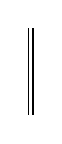
\begin{tikzpicture}\draw (0,0)--(0,1.1);\draw (.06,0)--(.06,1.1);\end{tikzpicture}}}\uline{Criterion of asphericity for a functor} f: C'$\hand{\to}$ C  between categories:
namely it is n. and s. that for any a $\hand{\in}$ Ob C,   $C'_{/a}$  be aspheric.

Let's come back to a \xout{would} category A,  for which we want to express
that it is a test-category,  namely for any \inserted{[small]} category B,  the natural
functor
\[ \hand{(*)} \qquad i_Aj_A(B) \hand{\longrightarrow} B \]
is a weak equivalence.  O\over{n}{n}e immediately checks that for any b$\hand{\in}$ Ob B,
the category  $i_Aj_A(B)_{/b}$ \xout{over} over $B_{/b}$  is isomorphic to $i_Aj_A(B_{/b})$ . Hence
we get the following
\uline{Proposition}  For a \inserted{[small]} category A,  the following are equivalent:
(i)  A is a test category,  namely (*) is a\deleted{n} \inserted{weak} equivalence for any \inserted{[small]}
category B.
(ii)  (*) is aspheric for any \inserted{[small]} category B.
(iii)  $i_Aj_A(B)$ is aspheric for any category B with final element.

This latter condition,  which is the most ``concrete'' one so far,
means also that the element
\[ F = j_A(B) = (\ a \hand{\mapsto} \mathrm{Hom}(\underset{\hand{\wedge}}{A}_{/a},B)) \hand{\in} \overset{\hand{\wedge}}{A} \]
is \deleted{an} \inserted[typed]{aspheric} \deleted{\xout{aspheric}} element of the topos $\overset{\hand{\wedge}}{A}$ ,  namely  the induced topos $\overset{\hand{\wedge}}{A}_{/F}$ is
aspheric (i.e. the category $A_{/F}$  is aspheric),  \uline{whenever} B has a final
element.

\hand{31.}  For the notion of a test category to make at all a sense,  we should
make sure in the long last that \hand{$\Delta$} itself,  the category of standar\over{t}{d} simpli-%
ces,  is indeed a test category.  So I finally set out to prove at least
\margin{$\times$} that much,  using the few reflexes I ha\over{d}{v}e in semi-simplicial homotopy theo\xout{r}-%
ry.  A proof finally peeled out it seems,  giving clues for handy conditi-%
ons in the general case,  which should be \uline{sufficient} \over{\unsure{in the base}}{at least} to insure
that B is a test category,  but maybe not quite necessary.  I'll try now
to get it down explicitly.
